\documentclass[10pt,a4paper,oneside]{scrartcl}

% Linking.
\usepackage{url}
\usepackage[unicode=true,colorlinks=false, pdfborder={0 0 0}]{hyperref}

% Language.
\usepackage[english]{babel}
\usepackage{csquotes}

% Bib Latex.
\usepackage[style=numeric,backend=bibtex]{biblatex}
\addbibresource{bibliography.bib}

% Better use of margins.
\usepackage[hmargin=2cm,vmargin=3cm]{geometry}

% Improves spacing for letters and numbers.
\usepackage{microtype}

% Fancy enumeration.
\usepackage{enumerate}

% Algorithms.
\usepackage{algorithm}
\usepackage[noend]{algpseudocode}

% Math stuff.
\usepackage[fleqn]{amsmath}
\usepackage{amssymb}
\usepackage{amsthm}
\usepackage{times}

\newtheorem{definition}{Definition}

% Allows the use of \includegraphics{...}.
\usepackage{graphicx}
\usepackage[center]{caption}
\usepackage{subcaption}

% Better tables.
\usepackage{tabularx}

% Uber table editor: http://truben.no/latex/table/

\begin{document}

%%%%%%%%%%%%%%%%%%%%%%%%%%%%%%%%%%%%%%%%%%%%%%%%%%%%%%%%%%%%%%%%%%%%%%%%%%%%%%%
% TTITLEPAGE
%%%%%%%%%%%%%%%%%%%%%%%%%%%%%%%%%%%%%%%%%%%%%%%%%%%%%%%%%%%%%%%%%%%%%%%%%%%%%%%
\title{Kung Fu Nao}
\subtitle{Human-Robot Interaction (MKI50)}

\author{ Bas Bootsma (0719080) \and Roland Meertens (3009653)}

\date{\today}

\maketitle

%%%%%%%%%%%%%%%%%%%%%%%%%%%%%%%%%%%%%%%%%%%%%%%%%%%%%%%%%%%%%%%%%%%%%%%%%%%%%%%
% INTRODUCTION
%%%%%%%%%%%%%%%%%%%%%%%%%%%%%%%%%%%%%%%%%%%%%%%%%%%%%%%%%%%%%%%%%%%%%%%%%%%%%%%
\section{Introduction}
Introducing the reader to the topic of learning from robots. 

The topic learning from demonstration is a topic that has seen a huge growth in the last few years.
This topic always consists of teaching a robot how to perform a task via demonstration by a human.  
A new topic is that of learning a human how to perform a task from demonstration by a robot. 

In this report an overview will be given of a robot capable of learning a human how to perform certain ``karate'' movements from demonstration by a robot. 
In this system a robot is able to perform a motion, teach the human how to perform this motion, assess the performance of the human and give extra information on the motions that are performed the worst by the user. 


%%%%%%%%%%%%%%%%%%%%%%%%%%%%%%%%%%%%%%%%%%%%%%%%%%%%%%%%%%%%%%%%%%%%%%%%%%%%%%%
% Hardware and Software
%%%%%%%%%%%%%%%%%%%%%%%%%%%%%%%%%%%%%%%%%%%%%%%%%%%%%%%%%%%%%%%%%%%%%%%%%%%%%%%
\section{Hardware and Software}

%%%%%%%%%%%%%%%%%%%%%%%%%%%%%%%%%%%%%%%%%%%%%%%%%%%%%%%%%%%%%%%%%%%%%%%%%%%%%%%
\subsection{Hardware}
In order to build this system the following components were used:
\begin{itemize}
  \item Laptop
  \item Nao robot
  \item Microsoft Kinect
\end{itemize}


%%%%%%%%%%%%%%%%%%%%%%%%%%%%%%%%%%%%%%%%%%%%%%%%%%%%%%%%%%%%%%%%%%%%%%%%%%%%%%%
\subsection{Software}
In order to program this system the following software has been used:
\begin{itemize}
  \item Microsoft visual studio 2012
  \item Microsoft Kinect SDK
  \item Choregraph
\end{itemize}


%%%%%%%%%%%%%%%%%%%%%%%%%%%%%%%%%%%%%%%%%%%%%%%%%%%%%%%%%%%%%%%%%%%%%%%%%%%%%%%
% System
%%%%%%%%%%%%%%%%%%%%%%%%%%%%%%%%%%%%%%%%%%%%%%%%%%%%%%%%%%%%%%%%%%%%%%%%%%%%%%%
\section{System}
Discuss the system from an AI point of view.

%%%%%%%%%%%%%%%%%%%%%%%%%%%%%%%%%%%%%%%%%%%%%%%%%%%%%%%%%%%%%%%%%%%%%%%%%%%%%%%
\subsection{Perception}
A way to detect the user and the body model. Do not mention the Kinect.

%%%%%%%%%%%%%%%%%%%%%%%%%%%%%%%%%%%%%%%%%%%%%%%%%%%%%%%%%%%%%%%%%%%%%%%%%%%%%%%
\subsection{Communication}
Gestures + speech...

%%%%%%%%%%%%%%%%%%%%%%%%%%%%%%%%%%%%%%%%%%%%%%%%%%%%%%%%%%%%%%%%%%%%%%%%%%%%%%%
\subsection{World Model}



%%%%%%%%%%%%%%%%%%%%%%%%%%%%%%%%%%%%%%%%%%%%%%%%%%%%%%%%%%%%%%%%%%%%%%%%%%%%%%%
% Individual Components
%%%%%%%%%%%%%%%%%%%%%%%%%%%%%%%%%%%%%%%%%%%%%%%%%%%%%%%%%%%%%%%%%%%%%%%%%%%%%%%
\section{Individual Components}

\subsection{Perception}
Skeleton tracking + dynamic time warping

%%%%%%%%%%%%%%%%%%%%%%%%%%%%%%%%%%%%%%%%%%%%%%%%%%%%%%%%%%%%%%%%%%%%%%%%%%%%%%%
\subsection{Communication}
Note here that we both use speech and gestures. 
Note that we use both beat gestures(gestures without semantic content) as well as metaphoric gestures (gestures indication thinking as well as gestures indication). 

The metaphoric gestures are:
\begin{itemize}
  \item Thinking
  \item Flexing of the muscles
  \item Bowing
\end{itemize}

%%%%%%%%%%%%%%%%%%%%%%%%%%%%%%%%%%%%%%%%%%%%%%%%%%%%%%%%%%%%%%%%%%%%%%%%%%%%%%%
\subsection{World Model}

%%%%%%%%%%%%%%%%%%%%%%%%%%%%%%%%%%%%%%%%%%%%%%%%%%%%%%%%%%%%%%%%%%%%%%%%%%%%%%%
\subsection{Graphical User Interface}



%%%%%%%%%%%%%%%%%%%%%%%%%%%%%%%%%%%%%%%%%%%%%%%%%%%%%%%%%%%%%%%%%%%%%%%%%%%%%%%
% Interaction
%%%%%%%%%%%%%%%%%%%%%%%%%%%%%%%%%%%%%%%%%%%%%%%%%%%%%%%%%%%%%%%%%%%%%%%%%%%%%%%
\section{Interaction Patterns}


\begin{figure}[h!]
	\caption{State diagram showing in what order the behaviours of the robot are performed}
	\centering
	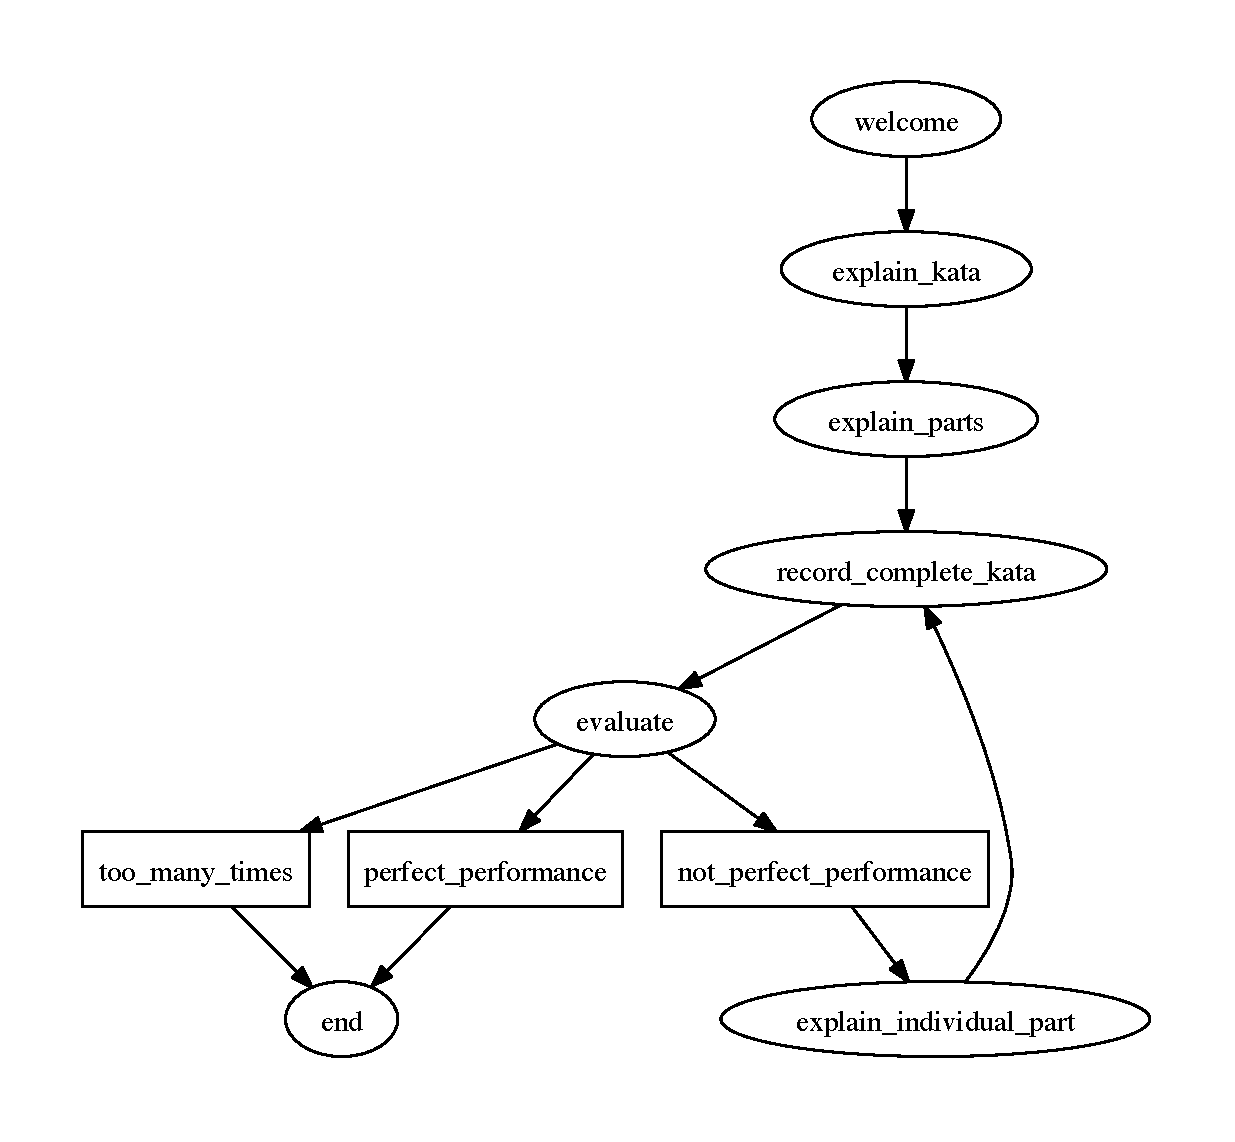
\includegraphics[width=0.5\textwidth]{images/stateDiagram}
	\label{fig:overviewTotalSystem}
\end{figure}


%%%%%%%%%%%%%%%%%%%%%%%%%%%%%%%%%%%%%%%%%%%%%%%%%%%%%%%%%%%%%%%%%%%%%%%%%%%%%%%
% Conclusion
%%%%%%%%%%%%%%%%%%%%%%%%%%%%%%%%%%%%%%%%%%%%%%%%%%%%%%%%%%%%%%%%%%%%%%%%%%%%%%%
\section{Conclusion}



%%%%%%%%%%%%%%%%%%%%%%%%%%%%%%%%%%%%%%%%%%%%%%%%%%%%%%%%%%%%%%%%%%%%%%%%%%%%%%%
% BIBLIOGRAPHY
%%%%%%%%%%%%%%%%%%%%%%%%%%%%%%%%%%%%%%%%%%%%%%%%%%%%%%%%%%%%%%%%%%%%%%%%%%%%%%%
\printbibliography

\end{document}
